\section{Modellering}

Att få fram ett bra E/R diagram till programmet är inte lätt. Man måste läsa beskrivningen av problemet som introducerats och analysera det in i minsta detalj för att sedan kunna skapa ett skapligt diagram. Vi satte och och läste texten några gånger och fick slutligen fram en någorlunda design. Efter att ha filat och gjort om skickade vi in den till projektansvarige för att få bekräftelse på om diagrammet ser bra ut eller om det behöver någon ändring. 

När vi fick tillbaka feedbacken var det enstaka punkter som korrigerades. Nu kunde vi övergå till relationsöversättning för att sedan kunna implementera databasen. E/R diagrammet syns på bilden nedan. 


\centerline{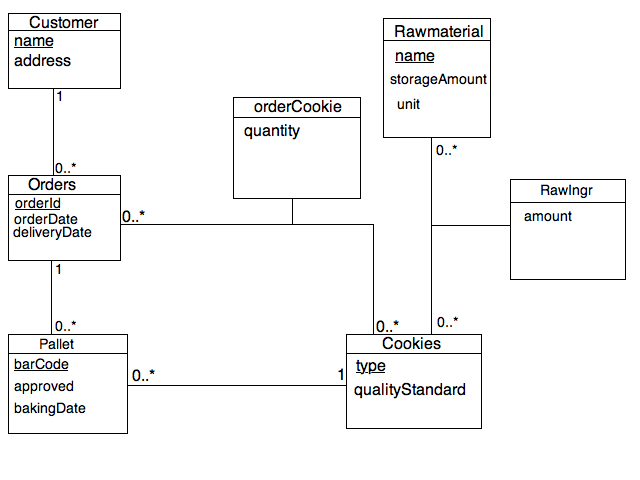
\includegraphics[scale = 0.6]{er.jpg}}